\documentclass[11pt]{article}

% use packages
\usepackage[utf8]{inputenc}
\usepackage{amsmath}
\usepackage{amsthm}
\usepackage{amsfonts}
\usepackage{amscd}
\usepackage{amssymb}
\usepackage{natbib}
\usepackage{url}
\usepackage[table,xcdraw,usenames]{xcolor}
%\usepackage[usenames]{color}

\usepackage{graphicx}
%\usepackage{mathtools}
\usepackage{enumitem}
\usepackage{authblk}
\usepackage{bm}


\usepackage{hyperref}
\usepackage{caption}
\usepackage{float}
\usepackage[caption = false]{subfig}
\usepackage{tikz}
\usepackage{multirow}
\usepackage[linesnumbered, ruled,vlined]{algorithm2e}
\usepackage{pdflscape}
\usepackage{etoolbox}
\AtBeginEnvironment{align}{\setcounter{equation}{0}} % https://tex.stackexchange.com/questions/349247/how-do-i-reset-the-counter-in-align

% margin setup
\usepackage{geometry}
\geometry{margin=0.8in}


% function definition
\newcommand{\R}{\mathbb{R}}
\newcommand{\w}{\textbf{w}}
\newcommand{\x}{\textbf{x}}
\newcommand{\dbf}{\textbf{d}}
\newcommand{\y}{\textbf{y}}
\newcommand{\X}{\textbf{X}}
\newcommand{\Y}{\textbf{Y}}
%\newcommand{\L}{\textbf{L}}
\newcommand{\Hist}{\mathcal{H}}
\newcommand{\Prob}{\mathbb{P}}
\def\mbf#1{\mathbf{#1}} % bold but not italic
\def\ind#1{\mathrm{1}(#1)} % indicator function
\newcommand{\simiid}{\stackrel{iid}{\sim}} %[] IID 
\def\where{\text{ where }} % where
\newcommand{\indep}{\perp \!\!\! \perp } % independent symbols
\def\cov#1#2{\mathrm{Cov}(#1, #2)} % covariance 
\def\mrm#1{\mathrm{#1}} % remove math
\newcommand{\reals}{\mathbb{R}} % Real number symbol
\def\t#1{\tilde{#1}} % tilde
\def\normal#1#2{\mathcal{N}(#1,#2)} % normal
\def\mbi#1{\boldsymbol{#1}} % Bold and italic (math bold italic)
\def\v#1{\mbi{#1}} % Vector notation
\def\mc#1{\mathcal{#1}} % mathical
\DeclareMathOperator*{\argmax}{arg\,max} % arg max
\DeclareMathOperator*{\argmin}{arg\,min} % arg min
\def\E{\mathbb{E}} % Expectation symbol
\def\mc#1{\mathcal{#1}}
\def\var#1{\mathrm{Var}(#1)} % Variance symbol
\def\checkmark{\tikz\fill[scale=0.4](0,.35) -- (.25,0) -- (1,.7) -- (.25,.15) -- cycle;} % checkmark
\newcommand\red[1]{{\color{red}#1}}
\def\bs#1{\boldsymbol{#1}}
\def\P{\mathbb{P}}
\def\var{\mathbf{Var}}
\def\naturals{\mathbb{N}}
\def\cp{\overset{p}{\to}}
\def\clt{\overset{\mathcal{L}^2}{\to}}

\setcounter{tocdepth}{4}
\setcounter{secnumdepth}{4}

\newtheorem{corollary}{Corollary}
\newcommand{\ceil}[1]{\lceil #1 \rceil}
\newcommand{\norm}[1]{\left\lVert#1\right\rVert} % A norm with 1 argument
\DeclareMathOperator{\Var}{Var} % Variance symbol

\newtheorem{cor}{Corollary}
\newtheorem{lem}{Lemma}
\newtheorem{thm}{Theorem}
\newtheorem{defn}{Definition}
\newtheorem{prop}{Proposition}
\theoremstyle{definition}
\newtheorem{remark}{Remark}
\hypersetup{
  linkcolor  = blue,
  citecolor  = blue,
  urlcolor   = blue,
  colorlinks = true,
} % color setup

% proof to proposition 
\newenvironment{proof-of-proposition}[1][{}]{\noindent{\bf
    Proof of Proposition {#1}}
  \hspace*{.5em}}{\qed\bigskip\\}
% general proof of corollary
  \newenvironment{proof-of-corollary}[1][{}]{\noindent{\bf
    Proof of Corollary {#1}}
  \hspace*{.5em}}{\qed\bigskip\\}
% general proof of lemma
  \newenvironment{proof-of-lemma}[1][{}]{\noindent{\bf
    Proof of Lemma {#1}}
  \hspace*{.5em}}{\qed\bigskip\\}

\allowdisplaybreaks

\title{Post-shock Volatility Forecasting Using Aggregated Shock Information}
\author{David Lundquist\thanks{davidl11@ilinois.edu} }
\affil{Department of Statistics, University of Illinois at Urbana-Champaign}
\date{December 3rd, 2021}

\begin{document}

\maketitle

\begin{abstract}
We develop a novel procedure for forecasting the volatility of a time series under study immediately following an exogenous news shock.  Adapting the synthetic prediction framework of \citet{lin2021minimizing}, we exploit series that have experienced similar shocks.  We extract volatility signals from these series in order to aggregate properly their shock-induced excess volatilities.  The volatility spikes are modeled as random effects and estimated as fixed effects.  The aggregation of these estimates is in service of adjusting the h-step-ahead GARCH forecast of the time series under study by an additive term.  The adjusted and unadjusted forecasts are evaluated using three families of benchmarks: the unobservable but easily estimated realized volatility (RV) of the time series under study, implied volatility, and the empirical volatility over horizons of varying length.  We also compare the performance of the adjusted forecast to the performance of the Realized GARCH forecast, which is known to react faster to rapidly changing volatility than the standard GARCH model by permitting the inclusion of metrics like implied volatility.   Finally, we combine Realized GARCH modeling with the synthetic prediction framework, using Realized GARCH in both the estimation of random effects as well as the forecast for the time series under study.  Real world illustrations are provided, as are simulation results suggesting the conditions under which our approach's hyperparameters can be tuned for best performance.
\end{abstract}


\section{Introduction}

The most important stochastic phenomenon of many time series $(P_{t})_{t\in\mathbb{N}}$, especially financial time series, is the volatility of the return series $(r_{t})_{t\in\mathbb{N}}$.  A financial asset's price series and daily return series may exhibit behavior that makes inconvenient and uninterpretable the traditional methods of time series analysis.  In contrast, the volatility of the return series may be less noisy, less structurally dependent on external factors, and more easily modeled as a weakly stationary process.  Yet even if one could model and forecast price series and return series with high accuracy, that would not necessarily tell us much about the variability of such forecasts nor enlighten us about the evolution of the variability of $(P_{t})_{t\in\mathbb{N}}$ over time. Modern portfolio management and theory requires information about at least the first two moments of a return series, if not higher.  For these reasons and others, volatility modeling has come to dominate financial econometrics over the past four decades.  

When $(P_{t})_{t\in\mathbb{N}}$ is positive, as one would expect of a price series, the percentage change over any interval of length $k\in\mathbb{N}$ can be approximated by $\text{log}(\frac{P_{t+k}}{P_{t}})$, owing to the fact that for any nonnegative real number y, $\text{log}(y+1)\leq y$.  Equality holds at exactly y = 0, corresponding to the case where $P_{t+k} = P_{t}$.  It is easily verified that the approximation works well when the ratio $\frac{P_{t+k}}{P_{t}} \in (.85,1.15)$, a return absolute value of $15\%$ or less.  The daily log return series $\text{log}(\frac{P_{t+1}}{P_{t}})$, however, not only provides an approximation to the daily return; the logarithm of a price series has the helpful property of being supported on $\mathbb{R}$.  Partly due to that, it earns a pedigree for its role in geometric Brownian motion, the foundation of much of modern financial mathematics, including the Black-Sholes differential equation \citep{tsay2005analysis}.  Additionally, the log transformation is a tried-and-true variance-reduction technique for heteroskedastic data \citep{faraway2016extending} and non-stationary time series.  In many applications, the log-return of a positive time series will allow us to reject the null of a unit-root process using the methods pioneered in \citet{dickey1979distribution} and \citet{dickey1981likelihood}, thus paving the way for the vast family of autoregressive-moving-average models.

However, no matter how a time series or its transformations is modeled, forecasting in the prescence of exogenous shock events requires a methodological framework that sensibly incorporates relevant information that has yet to manifest itself in market price or derivative quantities like volatility.  In this setting, regime-change models are of little use because under the assumption of a known exogenous shock, there is no need to estimate a regime-change time, nor is there data following the exogenous shock event to fit a model.  Asymmetric GARCH models were an early attempt to account for fact that negative returns typically beget larger volatility than positive returns \citep{hansen2012realized}.  As a separate problem, GARCH models have been shown slow to adapt to spikes in volatility (find first authors to point this out).  \citet{engle2002new} explored the use of implied volatility as an external regressor in a GARCH model, that is, using so-called GARCH-X models. \citet{hansen2012realized} propose Realized Garch, which aims to solve both the asymmetry problem as well as the slow-reaction problem by introducing a "measurement equation" as a tool for modeling the contribution to the conditional variance made by the market-implied volatility measure.  The key insight is that that the market-implied volatility measure is not independent of the conditional variance posited by the GARCH model.  Therefore, including the external measure must be done in a way that accounts for this dependence.

The approach herein can be viewed as an attempt to sidestep the functional complexity posited by Realized GARCH by substituting modeling assumptions.  Synthetic volatility forecasting proceeds under the assumption that similar exogenous shock events occasion volatility shocks arising from a common shock distribution.


\section{Setting}

\label{section2}

\begin{figure}[htbp]
  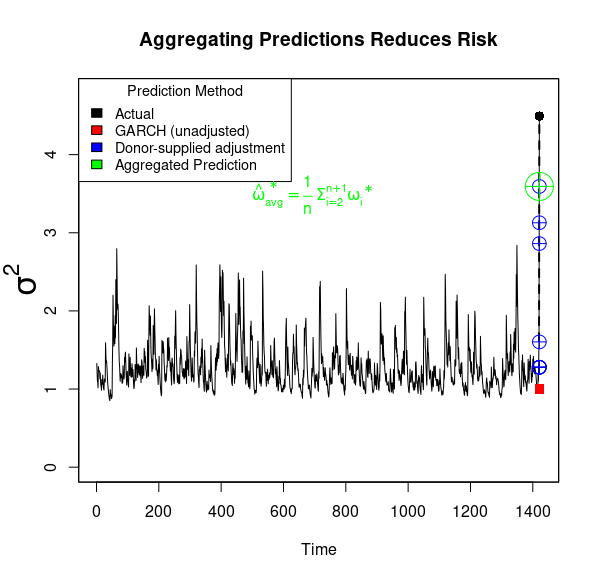
\includegraphics[scale=.5]{simulation_plots/plot_for_early_paper.png}
  \caption{An example of aggregating estimates using the arithmetic mean}
  \label{fig:arith_mean}
\end{figure}
Figure \ref{fig:arith_mean} shows a simple example.


We follow convention and define the daily log-return as $r_{t} = \text{log}(\frac{P_{t+1}}{P_{t}})$.  The class of ARIMA(p,d,q) models developed in the mid-to-late 20th century provides a framework for postulating and quantifying the autoregressive structure of $r_{t}$, all within the framework of frequentist statistics and maximum-likelihood estimation of parameters.  These models assume a certain dependence structure between $r_{t}$ and $(r_{k})_{k\leq t}$, as well as all observations in between, yet their errors -- often called innovations in the financial time series context due to how they represent the impact of new information -- are nevertheless assumed to be i.i.d. with mean zero and constant variance.  The ARCH \citep{engle1982autoregressive} and GARCH \citep{bollerslev1986generalized} models provide elegant alternatives to the constant-variance assumption.  In fact, the GARCH framework in its most basic form disregards $r_{t}$ and instead turns its interest to the series $r_{t}^{2}$ (when properly centered, i.e. after assuming a mean-model for returns).  

To that end, let $a_{t} = r_{t} - \mu_{t}$, where $\mu_{t}$ is the mean of the log return series $r_{t}$.  Implicitly, we are committing ourselves to a mean-model for $r_{t}$ in which $\mu_{t}$, the expected daily log-return, may vary with time, while $a_{t}$ is simply the noise.  As \citet{cont2001empirical} explains, such an assumption is justified by the empirical finding that returns lack significant autocorrelation.  We derive a mean-zero process $(a_{t})_{t\in\mathbb{N}}$ with the property that $\E[a^{2}_{t}] = \mrm{Var}[a_{t}]$.  Under the assumption of time-invariant volatility, the series $a_{t}^{2}$ should exhibit no autocorrelation at any lag $\ell\geq1$.  This assumption motivates tests for so-called ARCH effects, that is, tests for the clustering of volatility.  These tests explore the the alternative hypothesis that $\sigma_{t}^{2}$ is not only a time-varying parameter but furthermore a function of past squared residuals of the mean model.  In particular, the ARCH(m) model is an autoregressive model in which $\sigma_{t}^{2}$ is fitted using a linear combination of the $m$ past values of $a_{t}^{2}$.  The GARCH(m,s) framework take this one step further but modeling $\sigma_{t}^{2}$ as a linear combination of the $m$ past $a_{t}^{2}$ values and well as the $s$ past values of $\sigma_{t}^{2}$.  In functional form,

\begin{align*}
&\sigma_{t}^{2} = \omega + \sum^{m}_{k=1}\alpha_{k}a^{2}_{t-k} + \sum_{j=1}^{s}\beta_{j}\sigma_{t-j}^{2}\\
&a_{t} = \sigma_{t}\epsilon_{t}
\end{align*}



Assuming further that $\sigma^{2}_{t}$ depends on a vector of exogenous covariates $\x_{t}$ (a so-called "GARCH-X"), we have

\begin{align*}
&\sigma_{t}^{2} = \omega+ \sum^{m}_{k=1}\alpha_{k}a^{2}_{t-k} + \sum_{j=1}^{s}\beta_{j}\sigma_{t-j}^{2} + \gamma^{T}\x_{t}\\
&a_{t} = \sigma_{t}\epsilon_{t}
\end{align*}


We will suppose that a researcher has multivariate time series data $\y_{i,t}$, $t = 1, \ldots,  T_i$ and $i = 1, \ldots, n+1$. We let $\y_{i,t} = (y_{i,t}$, $\x_{i,t}$, $\textbf{v}_{i,t}$) where $y_{i,t}$ is a scalar response,  $\x_{i,t}$ is a vector of covariates that are revealed to the analyst prior to the observation of $y_{1,t}$, and $\textbf{v}_{i,t}$ is a vector of market-implied volatility metrics for the series $i$ that are available prior to the market open at time t.  Suppose that the analyst is interested in forecasting the volatility of $y_{1,t}$, the first time series in the collection.  We require that each time series $\y_{i,t}$ is subject to a news event immediately following $T^*_i \leq T_i + 1$ and before witnessing $T^*_i+1$. To define an interesting setting, we will suppose that $T^*_1 = T_1 + 1$, and $1 < T^*_i < T_i + 1$ for $i \geq 2$. 
We will suppose that $\x_{i,t=T^*_i}$ and $\textbf{v}_{i,t=T^*_i}$ are observed before the shock is manifested on $y_{i,t=T^*_i+1}$.

In light of the foregoing, we can rewrite the GARCH framework we are interested in as such

\begin{align*}
&\sigma_{i,t}^{2} = \omega_{i} + \sum^{m_{i}}_{k=1}\alpha_{i,k}a^{2}_{i,t-k} + \sum_{j=1}^{s_{i}}\beta_{i,j}\sigma_{i,t-j}^{2} + \gamma_{i}^{T} \begin{pmatrix} \x_{i,t} \\ \textbf{v}_{i,t} \\ \end{pmatrix} \\
&a_{i,t} = \sigma_{i,t}\epsilon_{i,t}
\end{align*}

% https://latex-tutorial.com/matrices-in-latex/
% https://www.math-linux.com/latex-26/faq/latex-faq/article/how-to-write-matrices-in-latex-matrix-pmatrix-bmatrix-vmatrix-vmatrix

We are interested in a multihorizon point forecast for $\sigma^{2}_{1,T^{*}+h}$, $h=1,2,...,H$, the h-step ahead conditional variance for the time series under study, up to a maximum forecast horizon of H.  The forecast performance evaluation uses three distinct loss functions, each computed using three families of estimators for the ground truth that we seek.  Let $L^{h}$ with the subscript "method, ground truth denote the loss function L and a pair, (prediction method, ground truth estimator), for an h-step-ahead forecast.  For example, a loss function of interest in this study is the 1-step-ahead MSE

$$ MSE^{1}_{synth pred, RV} = (\hat\sigma^{2}_{synth pred} - \hat\sigma^{2}_{RV})^{2}$$

In more generality, for an multihorizon volatility forecast with maximum forecast length H, the loss function is 

$$ MSE^{H}_{method, ground truth} = \frac{1}{H}\sum_{h=1}^{H}(\hat\sigma^{2}_{h, method} - \hat\sigma^{2}_{h, ground truth})^{2}$$

Also of interest in mean absolute-percentage-error for an h-step-ahead forecast, defined as

\[ 
\text{MAPE}^{H}_{method, ground truth} = \frac{1}{H}\sum_{h=1}^{H}\frac{|\hat\sigma^{2}_{h, method} - \hat\sigma^{2}_{h, ground truth}|}{\hat\sigma^{2}_{h, ground truth}}
\]

Finally, we introduce the QL (quasi-likelihood) Loss \citep{brownlees2011practical}:

\[ 
\text{QL}^{H}_{method, ground truth} = \frac{1}{h}\sum_{h=1}^{H} (\frac{ \hat\sigma^{2}_{h, method} }{\hat\sigma^{2}_{h, ground truth}} - \log{\frac{ \hat\sigma^{2}_{h, method} }{\hat\sigma^{2}_{h, ground truth}}} -1)
\]

What distinguishes QL Loss is that it is multiplicative rather than additive.  This serves as a basis for some of its virtues.  As \citet{brownlees2011practical} explains, "[a]mid volatility turmoil, large MSE
losses will be a consequence of high volatility without necessarily corresponding to
deterioration of forecasting ability. The QL avoids this ambiguity, making it easier to
compare losses across volatility regimes."

\subsection{Ground Truth Estimators}
\label{Ground Truth Estimators}

The price series of a financial asset is a sequence of observable random variables; in particular, for any $t$, $P_{t}$ is realized at $t$ and henceforth no longer random, under the assumption that $(P_{t})_{t\in\mathbb{N}}$ is adapted to $\mc{F}_{t}$.  Much of financial econometrics is devoted to decomposing $P_{t}$ into random and non-random components as well as understanding the covariance structure of $P_{t}$, difficult though that may be in some circumstances.  In contrast, the time-varying parameter $\sigma^{2}_{t}$ is a quantity for which even identifying an observable effect in the real world is far more challenging.  Approaches come in two basic forms: model-independent and model-dependent.  The naive approach of constructing a rolling unbiased estimator of the variance of a price series is analogous to using a rolling average to estimate the mean of a price series.  Implicitly, these approaches assume a simple, if unrealistic, covariance structure.  Additionally, they offer very little in the way of forward guidance (predictiveness) regarding the series at hand.  For that reason, in this section, we propose three families of estimators of the ground truth that we aim to forecast.

% https://tex.stackexchange.com/questions/186981/is-there-a-subsubsubsection-command
\subsubsection{Market-Implied Volatility}

Here we introduce implied volatility, a quantity that is derived using the equilibrium price of call and put options on the underlying financial asset.

We note also that Black-Scholes implied volatility is a biased estimator of volatility \citep{christensen1998relation}.

Find citation that Black-Scholes implied volatility is especially biased in times of a crisis.

\subsubsection{Realized Volatility}

Suppose we examine K units of of time, where each unit is divided into m intervals of length 1/m.  We follow the notation of  \citet{andersen2009realized}. Let $p_{t} = \text{log}(P_{t})$, and let $r(t, 1/m) = p_{t} - p_{t-1/m}$.  We estimate the variance of a log-return series using Realized Volatility, denoted $RV_{K,m}$, using

$$RV_{K,m} = \frac{1}{K}\sum^{Km}_{v=1}r^{2}(v/m,1/m)$$

Assuming that the K units $r(t, 1) = p_{t} - p_{t-1}$ are such that $r(t, 1) \simiid N(\mu, \delta^{2})$, it is easily verified that 

$$\E[RV_{K,m}] = \frac{\mu^{2}}{m} + \delta^{2}$$

which is a biased but consistent estimator of the variance.

\subsubsection{Historical Volatility}

As discussed in section 2, daily returns exhibit insigificant autocorrelation.  Such a finding could be used to motivate using the empirical volatility.  This is just the unbiased estimator of log-return $\sigma^{2}$ over the preceding M days.

\subsection{Volatility Profile of a Time Series}
\label{Volatility Profile of a Time Series}

In this section we make a novel contribution to the synthetic prediction framework by constructing a profile of a time series' volatility.  Suppose we have $D$ donors and for each of those $D$ donors, $q$ distinct measurements and/or covariates of volatility.  Abusing notation for RV ( I need some clever way to index (a) date, (b) donor, (c) how many days were used to get the measurement, we have...

\begin{equation*}
\textbf{V}_{q,D} = 
\begin{pmatrix}
\alpha_{T^{*},1} & \alpha_{T^{*},2}  & \cdots & \alpha_{T^{*},D}  \\
\beta_{T^{*},1} & \beta_{T^{*},2}  & \cdots & \beta_{T^{*},D}  \\
\vdots  & \vdots  & \ddots & \vdots  \\
RV_{T^{*},1} & RV_{T^{*},2}  & \cdots & RV_{T^{*},D}  \\
RV_{T^{*}-1,1}  & RV_{T^{*}-1,2}  & \cdots & RV_{T^{*}-1,D}  \\
\vdots  & \vdots  & \ddots & \vdots  \\
IV_{T^{*},1} & IV_{T^{*},2} & \cdots & IV_{T^{*},D} \\
IV_{T^{*}-1,1}  & IV_{T^{*}-1,2}  & \cdots & IV_{T^{*}-1,D} \\
\vdots  & \vdots  & \ddots & \vdots  \\
AbsoluteReturn_{T^{*},1} & AbsoluteReturn_{T^{*},2} & \cdots & AbsoluteReturn_{T^{*},D} \\
AbsoluteReturn_{T^{*}-1,1}  & AbsoluteReturn_{T^{*}-1,2}  & \cdots & AbsoluteReturn_{T^{*}-1,D} \\
\vdots  & \vdots  & \ddots & \vdots  \\
Volume_{T^{*},1}  & Volume_{T^{*},2}  & \cdots & Volume_{T^{*},D} \\
Volume_{T^{*}-1,1}  & Volume_{T^{*}-1,2}  & \cdots & Volume_{T^{*}-1,D}  \\
\vdots  & \vdots  & \ddots & \vdots  \\
\Delta RV_{T^{*},1} & \Delta RV_{T^{*},2}  & \cdots & \Delta RV_{T^{*},D}  \\
\Delta RV_{T^{*}-1,1}  & \Delta RV_{T^{*}-1,2}  & \cdots & \Delta RV_{T^{*}-1,D}  \\
\vdots  & \vdots  & \ddots & \vdots  \\
\end{pmatrix}
\end{equation*}


\subsection{Aggregation Mechanism}
\label{Aggregation Mechanism}

Here we explain how we use the volatility profile to arrive at a set of nonnegative weights that sum to 1.

In \citet{abadie2010synthetic}, the authors advance previous work in causal inference whereby a treatment effect can be estimated by creating a synthetic time series that that represents either the treatment or control unit.  The synthetic unit is constructed using a convex combination of so-called donor series.  The particular convex combination employed is a function of the distance between the time series under study and the donors. \citet{lin2021minimizing} adapt these methods for the purpose of prediction.  Their 1-step-ahead forecasts take inspiration from distance-based-weighting, pooling shock estimates from similar series according to the series' similarity to the series under study.  Their approach does not take into account the ARCH effects commonly observed in time series, especially financial times series, leaving unaccounted the variability that accompanies predictions of a heteroskedastic time series.  In this present study, we focus on only volatility forecasting.  We furthermore depart from the synthetic prediction framework by weighting series not by their covariates (which would be most appropriate for estimating the parameters of time series' mean model) but by their volatility profile.


\subsection{Model setup}
\label{modelsetup}
In this section, we will describe the assumed dynamic panel models for which 
post-shock aggregated estimators are provided. The basic structures of these models 
are the same for all time series in the analysis, the differences between them lie in the setup of the shock effect distribution.  We first sharply distinguish between a volatility shock induced by a return-series shock at time T*


\subsubsection{Volatility Shock Model}

Let $I(\cdot)$ be an indicator function, $T_i$ be the time length of the time series $i$ for $i = 1, \ldots, n+1$, and $T_i^*$ denote the largest time index prior to the arrival of the news shock , with $T_i^* < T_i$.  For $t= 1, \ldots, T_i$ and $i = 1, \ldots, n+1$, the model $\mc{M}_1$ is defined as

\begin{align}
\mc{M}_1 \colon &\sigma^{2}_{i,t} = \omega_{i} + \omega^{*}_i D^{vol}_{i,t} + \sum^{m_{i}}_{k=1}\alpha_{i,k}a^{2}_{i,t-k} + \sum_{j=1}^{s_{i}}\beta_{i,j}\sigma_{i,t-j}^{2} + \gamma_{i}^{T} \x_{i,t}\\
&a_{i,t} = \sigma_{i,t}(\epsilon_{i,t}(1-D^{level}_{i,t}) + \epsilon^{*}_{i}D^{level}_{i,t}) \label{equation1}
\end{align}

 where $D^{vol}_{i,t} = I(t \in \{T_i^* + 1,...,T_i^* + L_{i, vol}\})$, $D^{level}_{i,t} = I(t \in \{T_i^* + 1,...,T_i^* + L_{i, level}\})$ 
and $\x_{i,t} \in \R^{p}$ , with $p \geq 1$.  We assume that the 
$\mbf{x}_{i,t}$ are fixed.\footnote{Need to determine what difference it makes to a GARCH-X model, if any, for the covariates to be random.}\footnote{As for implied volatility as a covariate, the argument for regarding it as a non-random quantity is that we are not primarily concerned with what IV is trying to estimate.  We're concerned with IV itself as a primitive quantity that affects volitility through market sentiment. 'It is what it is.'}  For $i = 1, \ldots, n+1$ and $t=1, \ldots, T_i$, the random effects structure for $\mc{M}_1$ is:

\begin{align*}
\omega^{*}_i &\simiid \mc{F}_{\omega^{*}} \text{ with }  \; \mrm{E}_{\mc{F}_{\omega^{*}}}(\omega^{*}_i) = \mu_{\omega^{*}}, \mrm{Var}_{\mc{F}_{\omega^{*}}}(\omega^{*}_i)  = \sigma^2_{\omega^{*}}  \\
\epsilon^{*}_i &\simiid \mc{F}_{\epsilon^{*}} \text{ with }  \; \mrm{E}_{\mc{F}_{\epsilon^{*}}}(\epsilon^{*}_i) = \mu_{\epsilon^{*}}, \mrm{Var}_{\mc{F}_{\epsilon^{*}}}(\epsilon^{*}_i)  = \sigma^2_{\epsilon^{*}}  \\
% & \text{Alternatively, } (\omega^{*}, \epsilon^{*})_{i} \sim \mathcal{N}(\mu_{\omega^{*},\epsilon^{*}}, \Sigma_{\omega^{*},\epsilon^{*}}) \\
% THESE ARE NOT RANDOM &(\alpha, \beta)_i \simiid \mc{F}_{(\alpha, \beta)} \text{ where } \sum^{ \text{max} \{m,s \} }_{j}\alpha_j + \beta_j < 1 \\
% \mathbf{v}_i &\simiid \mc{F}_{\mathbf{v}} \text{ with }  \; \mrm{E}_{\mc{F}_{\mathbf{v}}}(\mathbf{v}_i) = \mu_{\mathbf{v}}, \mrm{Var}_{\mc{F}_{\mathbf{v}}}(\mathbf{v}_i)  = \Sigma^2_{\mathbf{v}} \\
\varepsilon_{i,t} & \simiid  \mc{F}_{\varepsilon} \text{ with }  \; \mrm{E}_{\mc{F}_{\varepsilon}}(\varepsilon_{i,t}) = 0, \mrm{Var}_{\mc{F}_{\varepsilon}}(\varepsilon_{i,t})  = 1 \\
%l_{i,vol} &\simiid \text{Unif}\{1,2,...,\text{maximum volatility shock length}\}\\
%l_{i, level} &\simiid \text{Unif}\{1,2,...,l_{i,vol}\}\\
\omega^{*}_{i} &\indep  \epsilon^{*}_i \indep \gamma_i \indep \varepsilon_{i,t}.
\end{align*}

\textbf{WHAT FOLLOWS IS (a) defense of the modeling choices, (b) remarks on the models' implications and subtleties}\\

The model $\mc{M}_1$ is defined by a volatility equation and mean equation, as is any GARCH model.  The choice to model the volatility shock $\omega^{*}_{i}$ as an additive random effect is straightforward.  However, the choice to model the level effect $\epsilon^{*}_{i,t}$ as a temporary rupture in the otherwise i.i.d. sequence of innovations $\epsilon_{i,t}$ stands in need of deeper justification.  One way of arguing for this choice is that, in a discrete time series model, if we assume the arrival of news in the time between $T^{*}$ and $T^{*}+1$, we do not have an easy way to express a conditional distribution of the innovation $\epsilon_{T^{*}+1}$ given the overnight arrival of information.  Using $\epsilon^{*}_{i,t}$ thus breaks this impasse.  This defense also explains why we do not parameterize the level shock at $T^{*}+1$ as a sum of two shocks, $\epsilon_{i,T^{*}+1}$ and $\epsilon^{*}_{i,T^{*}+1}$, which would represent the level shock as generated by two independent sources of stochasticity.  This would be inelegant and would also lack motivation as a practical level.  While we want to model the shock at $T^{*}+1$ as large in absolute value, we also want to retain the property of a unitary source of noise.

Note that under the popular GARCH(1,1), a dual level-volatility shock has an marginal effect on the conditional variance $\sigma^{2}_{i,t}$ that should be familiar to scholars of GARCH models.  As usual, assume $\alpha+\beta < 1$.  Furthermore, assume that both the volatility shock $\omega^{*}_{i}$ and the level shock $\epsilon^{*}_{i,t}$ are of length one only, and consider a circumstance with no exogenous regressor $\x_{i,t}$. Consider also the case where $r\geq 2$, which is necessary in order to isolate the effects of the level shock $\epsilon^{*}_{i,t}$.  Then

\begin{align}
\sigma^{2}_{i,T^{*}+r+1} & = \omega_{i} + \alpha_{i} a_{T^{*}+r}^{2} + \beta_{i}\sigma^{2}_{i,T^{*}+r} \\
& = \omega_{i} + \alpha_{i}(\sigma_{i,T^{*}+r}\epsilon_{T^{*}+r})^{2} + \beta_{i}\sigma^{2}_{i,T^{*}+r} \\
& = \omega_{i} + \sigma^{2}_{i,T^{*}+r}(\alpha_{i} (\epsilon_{T^{*}+r})^{2} + \beta_{i})
\end{align}

In (3), observe that $\omega_{i}^{*}$ and $\epsilon^{*}_{i,t}$ each appear at most once, through the term $\sigma^{2}_{T^{*}+r}$.  This might lead one to suspect  geometric decay of the shocks $\omega_{i}^{*}$ and $\epsilon^{*}_{i}$.  Such a suspicion is easier to substantiate by examining the conditional expectation of the variance, $\mathbb{E}[ \sigma^{2}_{i,T^{*}+r+1} |\mathcal{F}_{T^{*}+r}]$, which also happens to be the principal forecasting tool for a GARCH model.  Indeed, if we assume unit variance for all $\epsilon_{i,t}$ except, of course, $\epsilon^{*}_{i,t}$, then we have 

\begin{align*}
\mathbb{E}[ \sigma^{2}_{i,T^{*}+r+1} |\mathcal{F}_{T^{*}+r}] & = \mathbb{E}[\omega_{i} + \alpha a_{T^{*}+r}^{2} + \beta\sigma^{2}_{i,T^{*}+r} |\mathcal{F}_{T^{*}+r}] \\
& = \omega_{i} + \mathbb{E}[\alpha(\sigma_{i,T^{*}+r}\epsilon_{T^{*}+r})^{2} |\mathcal{F}_{T^{*}+r}] + \beta\sigma^{2}_{i,T^{*}+r} \\
& = \omega_{i} + \alpha\sigma_{i,T^{*}+r}^{2} + \beta\sigma^{2}_{i,T^{*}+r} \tag{Due to the unit variance assumption}\\
& = \omega_{i} + \sigma^{2}_{i,T^{*}+r}(\alpha + \beta) \\
\end{align*}

By repeated substitution, in conditional expectation, the shock is $\mathcal{O}((\alpha+\beta)^{r})$.  We generalize this observation in the following proposition.

\begin{prop}
Let $a_{t}$ be a mean-zero time series obeying a GARCH(1,1) specification prior to the arrival of a volatility shock of length $L_{\text{vol}} \geq 1$ and level shock of length $L_{\text{level}}\geq 1$ at some time $T^{*}+1$.  Then for any $r$ such that $r-1 \geq \text{max}\{L_{i, vol},L_{i, level}\}$, 

\begin{align}
\mathbb{E}[ \sigma^{2}_{i,T^{*}+r+1} |\mathcal{F}_{T^{*}+r}] & = \omega_{i} + \sigma^{2}_{i,T^{*}+r}(\alpha + \beta) \\
\end{align}
\end{prop}

\begin{proof-of-proposition}
We claim

\begin{align}
\mathbb{E}[ \sigma^{2}_{i,T^{*}+r+1} |\mathcal{F}_{T^{*}+r}] & = \mathbb{E}[\omega_{i} + \alpha a_{T^{*}+r}^{2} + \beta\sigma^{2}_{i,T^{*}+r} |\mathcal{F}_{T^{*}+r}] \\
& = \omega_{i} + \mathbb{E}[\alpha(\sigma_{i,T^{*}+r}\epsilon_{T^{*}+r})^{2} |\mathcal{F}_{T^{*}+r}] + \beta\sigma^{2}_{i,T^{*}+r} \\
& = \omega_{i} + \alpha\sigma_{i,T^{*}+r}^{2} + \beta\sigma^{2}_{i,T^{*}+r} \\
& = \omega_{i} + \sigma^{2}_{i,T^{*}+r}(\alpha + \beta) \\
\end{align}

The volatility equation of a GARCH(1,1) dictates that for any $r$, the one-step-ahead volatility is given by $\sigma^{2}_{i,T^{*}+r+1} = \omega_{i} + \alpha a_{i,T^{*}+r}^{2} + \beta\sigma^{2}_{i,T^{*}+r}$.  By the mean-model assumption of a GARCH(1,1), we have $a_{i,t} = \sigma_{i,t}\epsilon_{i,t}$.  By substitution, we arrive at equation (2) above.  Using the unit-variance assumption regarding $\epsilon_{T^{*}+r})$, we can compute explicitly the expectation in (2).  Finally, by rearranging terms, we arrive at equation (4).
\end{proof-of-proposition}


In other words, once two time points removed from the longest shock length, the volatility shock and level shock can be subsumed into one.  However, prior to being two time points removed, there is no such guarantee.  For example, one can take $r = 1$ and level shock of length at least one to see that 

\begin{align}
\mathbb{E}[ \sigma^{2}_{i,T^{*}+r+1} |\mathcal{F}_{T^{*}+r}] & = \mathbb{E}[\omega_{i} + \alpha a_{T^{*}+1}^{2} + \beta\sigma^{2}_{i,T^{*}+1} |\mathcal{F}_{T^{*}+1}] \\
& = \omega_{i} + \mathbb{E}[\alpha(\sigma_{i,T^{*}+r}\epsilon^{*}_{T^{*}+1})^{2} |\mathcal{F}_{T^{*}+1}] + \beta\sigma^{2}_{i,T^{*}+1} \\
& = \omega_{i} + \alpha\sigma^{2}_{i,T^{*}+1}(\mu^{2}_{\epsilon^{*}} + \sigma^{2}_{\epsilon^{*}}) + \beta\sigma^{2}_{i,T^{*}+1} \\
& = \omega_{i} + \sigma^{2}_{i,T^{*}+1}(\alpha(\mu^{2}_{\epsilon^{*}} + \sigma^{2}_{\epsilon^{*}}) + \beta)
\end{align}

 For each of the p entries in delta, the kth entry should have the property that
 
 $\mathbb{E}[ x_{i,t,k} * \delta_{k} ] > 0$
 
 In principle, you could have an M21 shock with a covariate that, in expectation, has a negative marginal contribution to the cumulative shock

Moreover, after both shocks have been exhausted, their influence disappears quickly.  This short-memory effect has implications for the method being developed herein:

\begin{enumerate}
\item Estimation of effects in donor pool should err on the side of underestimating, not overestimating, the length of the max shock, since overestimation of the shock length brings with it the risk of underestimating $\omega^{*}$.
\item An operator of the method needs some idea of how long the operator expects the shock in the time series under study to be.  Such an idea will guide her trust in the choice of k in the k-step ahead forecast the operator produces.  There are couple of obvious strategies: take all the donors, and over all the donor shock lengths, take the minimium.  Alternatively, one could take the maximum.
\item There may be different risks associated with over/underestimating level shock and vol shock lengths.
\end{enumerate}



In many settings, it is reasonable to model a volatility shock as occuring without a rupture in the mean-zero, i.i.d. sequence $\epsilon_{i,t}$.  In cases like this, outsize movement in the observable random variable $a_{i,t}$ is due solely to the shock $\omega_{i}^{*}$.  Using the ARMA representation of a GARCH(m,s) model, we can see clearly how the random effect $\omega_{i}^{*}$ increases the expectation of the nonnegative random variable $a_{i,t}^{2}$.  The unconditional mean of an ARMA model tells that the random effects simply contribute to the intercept term:

\begin{align*} 
\mathbb{E}[a^{2}_{i,t}] = \frac{\omega_{i} + \mathbb{E}[\omega_{i}^{*}] }{1 - \sum^{\text{max(m,s)}}_{k=1}(\alpha_{i,k}+\beta_{i,k})}
\end{align*} 

However, since it is not known a priori for which $t$ the effect $\omega_{i}^{*}$ will be nonzero, this fact is of little practical guidance.

\subsection{Why not parameterize the volatility shock as a change in coefficients?}
\begin{enumerate}
\item Swamped by shock: If the goal is near-term forecasting, then we don't really care how those coefficients may be changing.  The assumption is that if any changes occur, their influence cannot account for the large shock. Given that the GARCH parameters for a stationary GARCH process must sum to less than 1, there is an upper bound to the forecastable change.
\item Practically infeasible: If we did that, we would need quite a few time points to reliably estimate the change in the GARCH parameters.  We don't have that.
\end{enumerate}

\subsection{Improvements of this current work over its predecessor}
\begin{enumerate}
\item $y_{i,t}$ have shocks in both volatility and level.
\item The shocks can have length greater than 1.
\item The method under development does not strictly require knowledge of the length of the shocks in the donor pool, but correctly sizing up those shock lengths is helpful to proper estimation of the shocks.  However, an important question remains: even if the donor pool shock lengths are assumed to be known, how do we advise the operator to forecast the time series under study?  For how long is the forecast reliable?  Should we take a convex combination of the donor pool shock lengths?  Or mean? Or minimum of the donor pool shock lengths?
\item We may want a loss function that is asymmetric, i.e. penalizes upward and downward misses differently.
\item Lin+Eck 2021 requires exogenous information to arrive strictly between $T^{*}$ and $T^{*}+1$.  However, we may want to relax this requirement so as to permit the exogenous information to be concurrent with the trading session or end of session on $T^{*}+1$.
\item By offering more linear combination methods for the donor pool shocks (e.g. unit ball, affine hull, convex cone), we give the operator the ability to use donors such that the donor outcome series is negatively correlated with the time series under study.
\item See Tsay p. 94: if $t$ is the last index that has been observed, then our two-step-ahead forecast is made easier by rewriting the volatility equation as $\sigma^{2}_{i,t+1} = w_{i} + (\alpha_{i} + \beta_{i})\sigma^{2}_{i,t} + \alpha_{1}\sigma^{2}_{i,t}[\epsilon^{2}_{i,t} - 1]= w_{i} + (\alpha_{i} + \beta_{i})\sigma^{2}_{i,t} + \alpha_{1}\sigma^{2}_{i,t}[\epsilon^{2}_{i,t} - 1] $.  Usually, we assume unit variance (though not necessarily a N(0,1)).  However, what is the variance is smaller than 1?  Then in conditional expectation, the term $\alpha_{1}\sigma^{2}_{i,t}[\epsilon^{2}_{i,t} - 1]$ will be negative.  So it seems that for level shock, we want the signal to noise ratio to be large because the mean is high, not because the variance is low.
\end{enumerate}


Notice that $\mc{M}_1$ assumes that $\omega^{*}_i$ are i.i.d. with $\E[ \omega^{*}_i]=\mu_{\omega^{*}}$ 
for $i = 1, \ldots, n+1$. We also consider a model where the shock effects are linear functions of covariates with an additional additive mean-zero error. For $i = 1, \ldots, n+1$, the random effects structure for this model (model $\mc{M}_2$) is:

\begin{align}
\mc{M}_2 \colon \begin{array}{l}
   \sigma^{2}_{i,t} = \omega_{i} + \omega^{*}_i D_{i,t}  + \sum^{m_{i}}_{k=1}\alpha_{i,k}a^{2}_{i,t-k} + \sum_{j=1}^{s_{i}}\beta_{i,j}\sigma_{i,t-j}^{2} + \gamma_{i}^{T} \x_{i,t} \text{ }\\[.2cm]
   a_{i,t} = \sigma_{i,t}(\epsilon_{i,t}(1-D^{level}_{i,t}) + \epsilon^{*}_{i}D^{level}_{i,t})\\[.2cm]
   \omega_i^{*} = \mu_{\omega^{*}}+\delta'\mbf{x}_{i, T_i^*+1}+ \t{\varepsilon}_{i},
\end{array}\label{model2}
\end{align}

 where the added random effects are

\begin{align*}
\omega^{*}_i &\simiid \mc{F}_{\omega^{*}} \text{ with }  \; \mrm{E}_{\mc{F}_{\omega^{*}}}(\omega^{*}) = \mu_{\omega^{*}}, \mrm{Var}_{\mc{F}_{\omega^{*}_i}}(\omega^{*}_i)  = \sigma^2_{\omega^{*}}  \\
\epsilon^{*}_i &\simiid \mc{F}_{\epsilon^{*}} \text{ with }  \; \mrm{E}_{\mc{F}_{\epsilon^{*}}}(\epsilon^{*}_i) = \mu_{\epsilon^{*}}, \mrm{Var}_{\mc{F}_{\epsilon^{*}}}(\epsilon^{*}_i)  = \sigma^2_{\epsilon^{*}}  \\
% & \text{Alternatively, } (\omega^{*}, \epsilon^{*})_{i} \sim \mathcal{N}(\mu_{\omega^{*},\epsilon^{*}}, \Sigma_{\omega^{*},\epsilon^{*}}) \\
% THESE ARE NOT RANDOM &(\alpha, \beta)_i \simiid \mc{F}_{(\alpha, \beta)} \text{ where } \sum^{ \text{max} \{m,s \} }_{j}\alpha_j + \beta_j < 1 \\
\delta &\simiid \mc{F}_{\delta} \text{ with }  \; \mrm{E}_{\mc{F}_{\delta}}(\delta) = \mu_{\delta}, \mrm{Var}_{\mc{F}_{\delta}}(\delta_i)  = \Sigma_{\delta} \\
% \mathbf{v}_i &\simiid \mc{F}_{\mathbf{v}} \text{ with }  \; \mrm{E}_{\mc{F}_{\mathbf{v}}}(\mathbf{v}_i) = \mu_{\mathbf{v}}, \mrm{Var}_{\mc{F}_{\mathbf{v}}}(\mathbf{v}_i)  = \Sigma^2_{\mathbf{v}} \\
\varepsilon_{i,t} & \simiid  \mc{F}_{\varepsilon} \text{ with }  \; \mrm{E}_{\mc{F}_{\varepsilon}}(\varepsilon_{i,t}) = 0, \mrm{Var}_{\mc{F}_{\varepsilon}}(\varepsilon_{i,t})  = 1 \\
\t\varepsilon_{i} & \simiid  \mc{F}_{\t\varepsilon} \text{ with }  \; \mrm{E}_{\mc{F}_{\t\varepsilon}}(\t\varepsilon_{i}) = 0, \mrm{Var}_{\mc{F}_{\varepsilon}}(\varepsilon_{i})  = \sigma^2_{\t\varepsilon} \\
%l_{i,vol} &\simiid \text{Unif}\{1,2,...,\text{maximum volatility shock length}\}\\
%l_{i, level} &\simiid \text{Unif}\{1,2,...,l_{i,vol}\}\\
\omega^{*}_i &\indep  \epsilon^{*}_i \indep \gamma_i \indep \delta \indep \varepsilon_{i,t} \indep \t\varepsilon_{i}.
\end{align*}

\begin{table}[]
\begin{tabular}{|p{1.2in}|p{1.9in}|p{1.9in}|}
\hline
  & $\Sigma_{\delta} = I_{p}$ & $\Sigma_{\delta} \neq I_{p}$  \\ \hline
 $\Sigma_{x_{i,T^{*}}} = I_{p}$ & Easiest to model & Captures reasonable possibility of non-zero correlation in random effects \\ \hline
 $\Sigma_{x_{i,T^{*}}} \neq I_{p}$ & Captures empirically-verified phenomenon of non-zero correlation in covariates & Implausibly complicated to model  \\ \hline
\end{tabular}
\end{table}

\begin{table}[]
\begin{tabular}{|p{1.3in}|p{1.6in}|p{1.9in}|p{1.9in}|}
\hline
 & Vershynin (2018) & Lin and Eck (2021) & SynthVolForecasting \\ \hline
observed quantity& $y_{i}$  & NA & NA \\ \hline
estimated quantity&  NA& $\alpha_{i}$ &  $\omega^{*}_{i}$\\ \hline
signal & $A_{i}x$ & $\mu + \delta'x_{i,T^{*}}$ & $\mu + \delta'x_{i,T^{*}}$  \\ \hline
prior information & $x\in T$, $T$ a convex & across donors, linear shock function equal in distribution  &  across donors, linear shock function equal in distribution \\ \hline
key assumption(s) & $A_{i}$ independent $\forall i$, isotropic too? & $x_{i,T^{*}}$ independent across donors; independent entries of $x_{i,T^{*}}$ & $x_{i,T^{*}}$ independent across donors; independent entries of $x_{i,T^{*}}$ \\ \hline
noise& w & $\t\varepsilon$  & $\t\varepsilon$   \\ \hline
strategy& Observe $y_{i}$; then estimate $x$ with small expected L2 loss & Estimate $\alpha_{i}$ for $i = 2,...,n+1$; then take convex combination to predict $\alpha_{1}$  & Estimate $\omega^{*}_{i}$ for $i = 2,...,n+1$; then take convex combination to predict $\omega^{*}_{1}$ \\ \hline
\end{tabular}
\end{table}

We further define the parameter sets
\begin{align}
  \begin{array}{lll}
     \Theta &= &\{(\omega^{*}_i, \epsilon^{*}_i,\gamma_i, \delta,\varepsilon_{i,t},\t\varepsilon_{i})\colon t= 1, \ldots, T_i, i = 2, \ldots, n +1\},\\
    \Theta_1 &= &\{(\omega^{*}_i, \epsilon^{*}_i,\gamma_i, \delta,\varepsilon_{i,t},\t\varepsilon_{i})\colon t= 1, \ldots, T_i, i = 1\},\label{parameter}
  \end{array}
\end{align}
where $\Theta$ and $\Theta_1$ can be adapted to $\mc{M}_1$ by dropping $\delta$. We assume this for notational simplicity.

\subsection{Forecasting}

Here we make reference to Tsay p. 133 and explain, very similarly to Tsay, that the prediction function for a GARCH(m,s) is very similar to an ARMA prediction function.  Modeled after section 2.2 here https://arxiv.org/pdf/2008.11756.pdf

$\mathbb{E}[ \sigma^{2}_{i,T^{*}+r+1} |\mathcal{F}_{T^{*}+r}]$

\section{Simulation Setup and Results}

Having introduced the model parameters above, we introduce estimation techniques that can be varied

\begin{figure}
  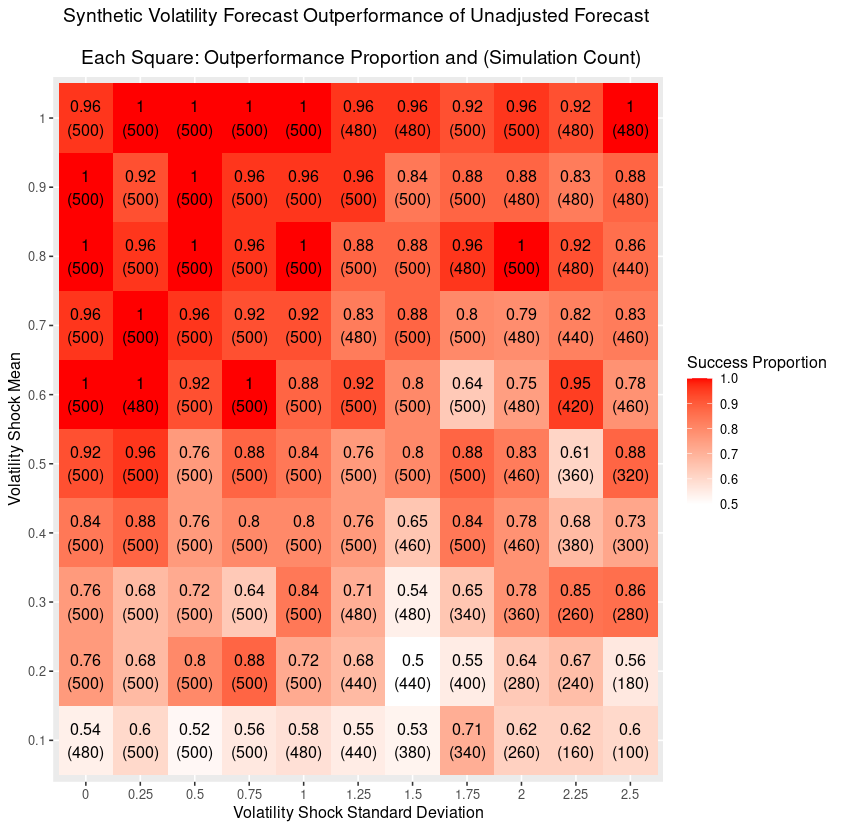
\includegraphics[scale=.5]{simulation_plots/outperformance_grid.png}
  \caption{An example of aggreation using arithmetic mean}
  \label{fig:arith_mean}
\end{figure}
Figure \ref{fig:arith_mean} shows a simple example.


\begin{enumerate}
  \item Additional measurement periods
  \item Optimization norm 
\end{enumerate}

We also introduce simulation parameters that can be varied but are not random effects

\begin{enumerate}
  \item Length of the volatility shock
  \item Length of the level shock
\end{enumerate}

\section{Connection to Signal Recovery}


\bibliographystyle{plainnat}
\bibliography{synthVolForecast}
%\bibliography{../synthetic-prediction-notes}

  
\end{document}


